% %%%%%%%%%%%%%%%%%%%%%%%%%%%%%%%%%%%%%%%%%%%%%%%%%%%%%%%%%%%%
% CHAPTER 4 - RESULTS AND DISCUSSION (guideline 2.4) ~20 pages
% Generated from Chapter4.src.tex: review-ID citations (\pc, \tc, \pcs)
% are converted to biblatex citations with verified first pages.
% Evidence coded from abstracts (see SLR_Search_and_Screening.xlsx).
% %%%%%%%%%%%%%%%%%%%%%%%%%%%%%%%%%%%%%%%%%%%%%%%%%%%%%%%%%%%%

\chapter{Results and Discussion}
\label{ch:results}

This chapter presents the results of the systematic literature review. Section~\ref{sec:study-characteristics} describes the characteristics of the 109 included studies. Sections~\ref{sec:results-ai-ca} to~\ref{sec:mediation} synthesise the evidence along the research questions: the link between AI capabilities and competitive advantage, the role of sensing, seizing and transforming, and the mediating role of dynamic capabilities. Section~\ref{sec:proposition-evaluation} evaluates the three research propositions, and Section~\ref{sec:discussion} discusses the findings in light of the theoretical framework developed in Chapter~\ref{ch:literature}. Unless stated otherwise, the findings refer to the final, adjudicated coding described in Section~\ref{sec:data-extraction}, which is based on the abstracts and, for the 29 studies whose full text could be accessed, on the full text.

% ------------------------------------------------------------
\section{Literature Search and Study Characteristics}
\label{sec:study-characteristics}

The review includes 109 studies, which are listed individually in Appendix~\ref{AppendixB}. Table~\ref{tab:publication-characteristics} summarises their main characteristics. The most striking feature of the evidence base is its recency. Only 15 studies were published between 2020 and 2023, whereas 13 appeared in 2024, 23 in 2025 and 58 in 2026, including articles published online ahead of print. Almost three quarters of the evidence is therefore less than two years old. This confirms the observation in Chapter~\ref{ch:literature} that research on AI capabilities is a young and rapidly growing field, but it also means that many findings have not yet been replicated or debated in subsequent work.

Of the included studies, 18 are core studies set in e-commerce, online retail or platform-based businesses, and 91 are supporting studies from other industries. The supporting studies cover a wide range of contexts, most frequently manufacturing, small and medium-sized enterprises, banking and financial services, hospitality, supply chains and start-ups. The predominance of supporting studies underlines that the e-commerce-specific evidence on AI capabilities and competitive advantage is still limited, which is consistent with research gap G1 (Table~\ref{tab:gaps}).

\begin{table}[H]
  \centering
  \caption{Publication Characteristics of Included Studies}
  \label{tab:publication-characteristics}
  \small\setstretch{1.0}\sloppy
  \begin{tabularx}{\textwidth}{>{\raggedright\arraybackslash}p{3.2cm}>{\raggedright\arraybackslash}X>{\raggedleft\arraybackslash}p{1.2cm}}
    \toprule
    \textbf{Characteristic} & \textbf{Category} & \textbf{n} \\
    \midrule
    Publication year & 2020--2023 / 2024 / 2025 / 2026 & 15 / 13 / 23 / 58 \\
    \addlinespace
    Tier & Core (e-commerce, online retail, platforms) / supporting & 18 / 91 \\
    \addlinespace
    Research design & Survey (mostly PLS-SEM) & 56 \\
     & Conceptual & 16 \\
     & Mixed methods & 15 \\
     & Qualitative and case studies & 13 \\
     & Panel or archival data & 7 \\
     & Formal (game-theoretic) models & 2 \\
    \addlinespace
    Region (where reported; multiple possible) & China & 17 \\
     & South and South-East Asia (e.g.\ India, Pakistan, Vietnam) & 14 \\
     & Middle East and North Africa (e.g.\ Saudi Arabia, Jordan, Egypt) & 13 \\
     & Europe & 8 \\
     & North America & 5 \\
     & Other (e.g.\ Taiwan, Hong Kong, Australia, multi-country) & 7 \\
     & Not reported in the abstract & 47 \\
    \addlinespace
    Theoretical lens & Dynamic capabilities / RBV / both / none named & 56 / 27 / 14 / 30 \\
    \addlinespace
    Journal & Listed in the VHB Rating 2024 & 56 \\
    \addlinespace
    Quality (Table~\ref{tab:quality}, Q1--Q6) & High (6) / medium (4--5) / low (0--3) & 53 / 45 / 11 \\
    \addlinespace
    Limitations discussed (Q7) & Yes / no / not assessable & 34 / 8 / 67 \\
    \addlinespace
    Evidence source & Full text verified / abstract only & 37 / 72 \\
    \bottomrule
  \end{tabularx}
  \source{Author's own work based on the data extraction}
\end{table}

Methodologically, the evidence is dominated by cross-sectional surveys of managers, most of them analysed with partial least squares structural equation modelling. Conceptual studies form the second largest group, followed by qualitative case studies. Panel studies based on archival data are rare and are concentrated in China \parencites[1]{slrR010}[1]{huang2026}[1]{dai2026}. Only a handful of studies use designs that observe firms over time, such as a three-wave survey of Vietnamese start-ups \parencite[1]{slrR037} or a time-lagged survey in Saudi retail and e-commerce \parencite[1]{slrR111}. Geographically, the evidence comes mainly from China, the Middle East and South Asia. Only eight studies refer to European firms, and none of the studies that report their context is set in Germany. For a thesis written in Germany, this is an important limitation of the transferability of the findings, which is taken up again in Section~\ref{sec:discussion}.

Dynamic capabilities theory is the most frequently used theoretical lens: 56 studies refer to it explicitly, 27 to the resource-based view and 14 combine both perspectives. At the same time, 30 studies do not name a theoretical foundation in their abstract. According to the quality assessment on criteria Q1 to Q6, 53 studies were rated as high quality, 45 as medium quality and 11 as low quality, with a mean score of 5.1 out of 6. Whether limitations are discussed (Q7) could be assessed for only 42 studies: 34 of them discuss their limitations and eight do not, while for the remaining 67 studies this criterion is not assessable from the abstract and is therefore reported separately rather than scored as zero. Quality is not related to the journal listing: among the 56 studies in VHB-listed journals, 26 were rated as high quality, compared with 27 of the 53 studies in non-listed journals. The studies are spread across a large number of journals, and no single outlet dominates. The most frequent outlets are \emph{Strategic Business Research} (seven studies), \emph{Industrial Marketing Management} and the \emph{International Journal of Information Management} (five each), the \emph{Journal of Business Research} (four) and the \emph{Academy of Management Review} (three). This dispersion reflects the interdisciplinary nature of the topic, which connects strategic management, information systems, marketing and operations research.

Figure~\ref{fig:themes} shows how the studies are distributed across outcome types. Firm performance is the most frequently studied outcome (32 studies), followed by competitive advantage (23 studies). Firm performance was coded separately and was not treated as competitive advantage, and competitive advantage was only coded as sustainable when the authors explicitly framed it as sustained or long-term. On this basis, only 11 studies examine sustainable competitive advantage or a comparable long-term outcome, and none of these is a core study from e-commerce or platform contexts. Further studies address innovation outcomes, including new product performance (11), resilience (8) and business model innovation (6), while 18 studies examine other outcomes such as strategic renewal, user value or implementation success.

\begin{figure}[H]
  \centering
  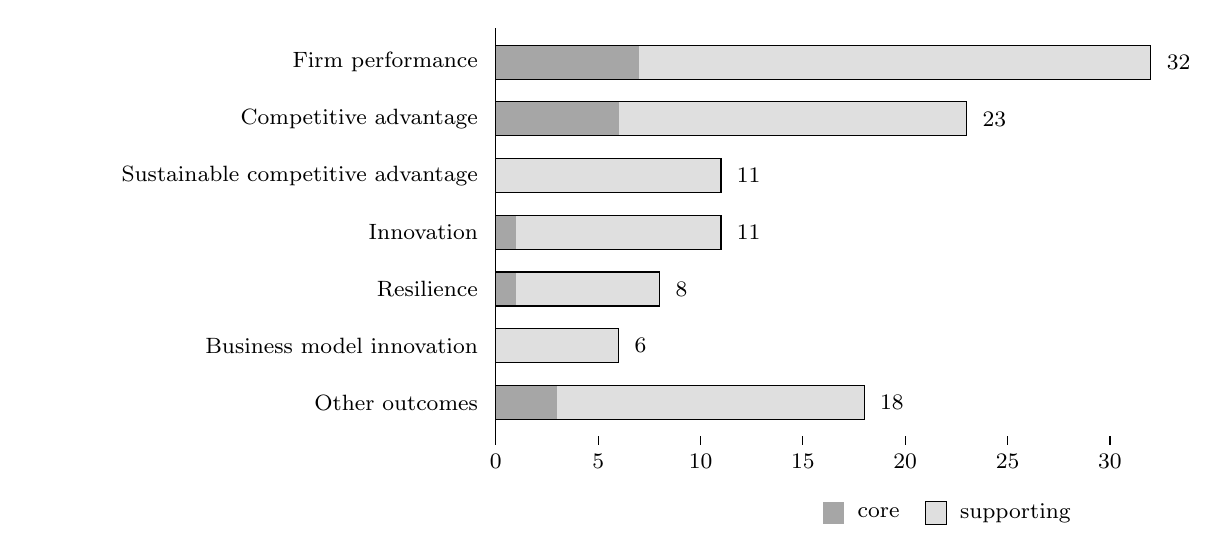
\begin{tikzpicture}[font=\footnotesize, x=0.26cm, y=0.72cm]
    % bars: core (dark) + supporting (light); values from the data extraction
    \foreach \lab/\c/\s/\y in {Firm performance/7/25/7, Competitive advantage/6/17/6, Sustainable competitive advantage/0/11/5, Innovation/1/10/4, Resilience/1/7/3, Business model innovation/0/6/2, Other outcomes/3/15/1} {
      \node[anchor=east, align=right, text width=5.6cm] at (-0.4,\y) {\lab};
      \fill[gray!70] (0,\y-0.3) rectangle (\c,\y+0.3);
      \fill[gray!25] (\c,\y-0.3) rectangle (\c+\s,\y+0.3);
      \draw (0,\y-0.3) rectangle (\c+\s,\y+0.3);
      \pgfmathtruncatemacro{\tot}{\c+\s}
      \node[anchor=west] at (\c+\s+0.3,\y) {\tot};
    }
    \draw (0,0.4) -- (0,7.6);
    \foreach \t in {0,5,10,15,20,25,30} {\draw (\t,0.4) -- (\t,0.25) node[below] {\t};}
    \fill[gray!70] (16,-1.15) rectangle (17,-0.75); \node[anchor=west] at (17.2,-0.95) {core};
    \fill[gray!25] (21,-1.15) rectangle (22,-0.75); \draw (21,-1.15) rectangle (22,-0.75); \node[anchor=west] at (22.2,-0.95) {supporting};
  \end{tikzpicture}
  \caption{Distribution of Studies by Research Theme}
  \label{fig:themes}
  \source{Author's own work based on the data extraction (n = 109)}
\end{figure}

% ------------------------------------------------------------
\section{AI Capabilities and Competitive Advantage}
\label{sec:results-ai-ca}

The first research question asks how AI capabilities are associated with competitive advantage. Of the 109 studies, 79 provide evidence on this link. In 63 of them, AI capabilities are positively associated with competitive advantage, firm performance or innovation outcomes, nine studies describe the relationship as conditional, five find no significant direct effect and two highlight constraints that prevent firms from turning AI into an advantage. For the remaining 30 studies the evidence is insufficient, either because they examine other outcomes or, in one case, because the abstract does not report the direction of the effect \parencite[205]{chatterjee2021}. Table~\ref{tab:evidence-ca} summarises this evidence by outcome type.

\begin{table}[H]
  \centering
  \caption{Evidence Linking AI Capabilities to Competitive Advantage}
  \label{tab:evidence-ca}
  \small\setstretch{1.0}\sloppy
  \begin{tabularx}{\textwidth}{>{\raggedright\arraybackslash}p{2.6cm}>{\centering\arraybackslash}p{1.1cm}>{\raggedright\arraybackslash}p{3.2cm}>{\raggedright\arraybackslash}X}
    \toprule
    \textbf{Outcome type} & \textbf{n} & \textbf{Direction of evidence} & \textbf{Representative studies} \\
    \midrule
    Firm performance & 32 & 29 positive, 3 n.s.\ direct effect & Core: \parencites[1]{chen2022}[1]{slrR111}[93]{slrR219}; supporting: \parencites[1]{mikalef2021capability}[1]{fossowamba2022}[1]{slrR079}[1]{slrR120} \\
    \addlinespace
    Competitive advantage & 23 & 16 positive, 5 conditional, 1 constraint, 1 insufficient & Core: \parencites[1]{bunea2026}[1]{slrR228}[1250]{slrR216}[187]{chen2026}; supporting: \parencites[1]{slrR030}[1]{slrR041}[10]{li2025}[1425]{krakowski2023} \\
    \addlinespace
    Sustainable competitive advantage & 11 & 6 positive, 2 n.s., 2 conditional, 1 constraint & Supporting only: \parencites[1]{liang2026}[240]{hossain2022}[1]{slrR003}[1]{wu2026}[1]{slrR077} \\
    \addlinespace
    Innovation (incl.\ new product performance) & 11 & 10 positive, 1 conditional & \parencites[1]{slrR022}[84]{dinh2026}[44]{slrR123}[1]{slrR010} \\
    \addlinespace
    Resilience, business models & 14 & Link to advantage rarely tested & \parencites[1]{dai2026}[1]{slrR096}[574]{sjodin2021}[1]{slrR083} \\
    \bottomrule
  \end{tabularx}
  \source{Author's own work based on the data extraction; n.s.\ = not significant}
\end{table}

The core studies from e-commerce consistently report positive associations, but mostly with performance rather than with competitive advantage in the strict sense. In a survey of 394 e-commerce firms, AI capability affects firm performance only indirectly, through creativity, AI management and AI-driven decision making \parencite[1]{chen2022}. In Saudi retail and e-commerce, AI capability contributes to organisational performance by facilitating service innovation and improved consumer outcomes, with digital infrastructure acting as a supporting factor \parencite[1]{slrR111}. A survey of e-commerce managers examines how the use of generative AI builds technological capabilities that are linked to financial performance in terms of sales, revenue and profitability \parencite[93]{slrR219}, and in Saudi SMEs the adoption of AI in e-commerce enhances business performance \parencite[1]{aljarboa2024}. Operational benefits are reported as well: AI usage improves the logistics efficiency of Indian e-commerce businesses, partly through supply chain consistency and last-mile delivery performance \parencite[290]{slrR241}, and qualitative evidence from Philippine clothing retailers shows that even free AI tools improve management, targeted advertising and customer communication \parencite[76]{slrR193}.

Further core studies extend this picture to marketing and to cross-functional effects. In Egyptian e-retail stores, AI applications are strongly correlated with marketing innovation, with organisational culture acting as a mediator \parencite[170]{slrR242}. A survey of 750 business managers, financial executives and e-commerce practitioners conceptualises AI adoption as a cross-functional capability and finds consistent positive effects on business management, e-commerce and finance \parencite[1]{slrR184}. A literature-based conceptual study describes personalisation, predictive analytics and automation as the core AI capabilities that transform marketing in e-business environments, with customer engagement and satisfaction linking these capabilities to marketing outcomes \parencite[1]{slrR155}. These studies confirm that, in e-commerce, the benefits of AI are closely tied to customer-facing processes, but they also rely on correlational or conceptual evidence.

Only a few core studies measure competitive advantage directly. In electronic retailing, AI implementation is associated with qualitative and quantitative benefits that are linked, through customer experience, to differentiation- and cost-based competitive advantage \parencite[1]{bunea2026}. Among Jordanian e-commerce firms, IT capabilities mediate the relationship between AI and competitive advantage \parencite[1]{slrR228}, and for Chinese SMEs on cross-border platforms, the coupling of AI adoption and strategic agility improves their position in global value chains through international marketing capabilities \parencite[1250]{slrR216}. Platform-specific theory points in the same direction but emphasises dynamics: the AI capability of a platform increases the value users perceive through data network effects \parencite[534]{gregory2021}, and an entrant with a superior algorithm can overcome an incumbent's user base \parencite[187]{chen2026}. A game-theoretic study of live streaming shows, however, that the competitive advantage of an online retailer depends on conditions such as online acceptance and the relative advantage of human-hosted or AI-supported streaming \parencite[1348]{slrR199}.

Two further core studies and one related supporting study conceptualise how AI creates advantage at the level of platforms and ecosystems rather than individual firms. One framework explains how AI-based capabilities are translated into dynamic competitive positioning through strategic intelligence, the orchestration of platform ecosystems and network effects \parencite[649]{slrR088}. In solution-based business models of manufacturers, AI platforms are argued to foster collaborative value systems between firms and other value-chain actors across problem identification, solution development and implementation, and thereby to support the development of situating capabilities \parencite[1]{slrR179}. At the level of multinational enterprises, orchestration theory proposes that firms create value by orchestrating globally distributed resources and partners within digital platform and AI ecosystems \parencite[689]{slrR213}. These contributions shift the unit of analysis from the firm to the ecosystem: in platform-based business, AI capabilities may create advantage less through internal efficiency than through the ability to coordinate external actors and to learn from the data they generate. Since these studies are conceptual or do not test competitive advantage directly, however, these arguments still await empirical testing.

The supporting studies confirm the positive association across many industries. AI capabilities increase competitive advantage in Jordanian manufacturing firms, partly through organisational agility \parencite[1]{slrR030}, in micro, small and medium-sized enterprises through supply chain agility and resilience \parencite[1]{slrR041}, and in B2B firms through service innovation \parencite[10]{li2025}. Comparable results are reported for hotels \parencite[1]{slrR108}, Vietnamese SMEs \parencite[1]{slrR053}, multinational corporations \parencite[1]{slrR006} and Tunisian family firms \parencite[1]{slrR075}. In customer-facing functions, one study examines how AI-based CRM relates to performance and competitive advantage depending on firm size, age and industry, although its abstract does not report the direction of the effects \parencite[205]{chatterjee2021}, and an AI-powered CRM capability improves profitability and competitive advantage through marketing ambidexterity \parencite[1]{alnofeli2026}.

Across industries, the supporting studies reveal recurring patterns that are relevant for e-commerce. In manufacturing, AI capabilities are mainly linked to innovation and to new service-based business models: they foster servitization, especially when absorptive capacity is high \parencite[1]{slrR017}, improve the novelty and efficiency of business model design \parencite[1]{slrR083} and support product and new product performance \parencites[1]{slrR131}[44]{slrR123}. In hospitality, AI capabilities create advantage through supply chain agility and resilience \parencite[1]{slrR108} and through co-innovation \parencite[2055]{slrR174}. In banking and financial services, AI-enabled risk analytics \parencite[1]{slrR122} and AI-powered CRM \parencite[1]{alnofeli2026} are linked to financial performance and competitive advantage. Studies of SMEs and start-ups emphasise agility and business model change, but also resource constraints \parencites[1]{slrR053}[1]{slrR091}[1]{slrR037}. Several of these mechanisms, in particular customer relationship management, service innovation, supply chain agility and business model change, are central to e-commerce as well. This supports the transferability of the supporting evidence, while the specific role of data network effects and platform competition can only be assessed from the core studies.

The 11 studies that address sustainable competitive advantage deserve particular attention, because this outcome is at the centre of the thesis. Six of them are conceptual. One proposes that AI-driven strategic capabilities, such as AI-enabled market intelligence and AI governance, lead to sustainable competitive advantage through an organisational sustainability capability that enables firms to sense, seize and realign their resources \parencite[1]{slrR001}. Another links AI-driven capabilities, embedded sustainability and adaptive organisational cultures to durable advantage \parencite[1]{slrR026}, and a third develops a framework for AI-driven branding aimed at sustained brand advantage \parencite[1]{slrR170}. Empirically, a marketing analytics capability helps exporters sense, seize and reconfigure the market, leading to a sustained competitive advantage, and AI adoption strengthens these capabilities \parencite[240]{hossain2022}. Panel data from Chinese listed firms show that AI helps firms balance short-term returns and long-term growth through organisational resilience and strategic change \parencite[1]{liang2026}, and AI capability maturity is linked to competitive performance framed as sustained advantage through human-AI integration and marketing agility \parencite[1]{slrR149}. In contrast, the direct effect of AI capabilities on sustainable competitive advantage is not significant in Spanish high-growth industries \parencite[1]{slrR003}, the full text of a study of Chinese high-tech firms shows that AI capability neither has a significant main effect on sustainable competitive performance nor moderates the effect of disruptive innovation \parencite[1]{slrR059}, democratised generative AI is argued to yield a sustained advantage only for firms that build proprietary perceptual systems \parencite[583]{cui2024}, small businesses often fail to achieve a lasting advantage from AI \parencite[1]{slrR077}, and whether AI produces fleeting efficiency gains or sustained advantages depends on how managers frame it \parencite[1]{wu2026}. The evidence on sustainability is therefore thin, comes exclusively from supporting studies and relies mostly on conceptual reasoning or on managers' perceptions rather than on observed persistence of advantage.

A closer look at the remaining studies reveals that a direct effect of AI capabilities on competitive outcomes is not the rule. In five studies, the direct link is not significant. In Spanish high-growth industries, digital transformation leadership affects sustainable competitive advantage, whereas the direct effect of AI capabilities is not significant \parencite[1]{slrR003}, and in Chinese high-tech firms AI capability has no significant main effect on sustainable competitive performance \parencite[1]{slrR059}. A reanalysis of SME data finds no significant direct link between AI capability and performance, but a positive indirect effect through AI adoption and dynamic capabilities \parencite[1]{slrR011}. In early-stage ventures, strategic resilience fully accounts for the relationship between AI capability and entrepreneurial success \parencite[1]{wang2026}, and in B2B loyalty programmes, the direct effect of AI capability on performance is weak and not significant, while three quarters of the total effect run through customer-relating capability and programme adaptation \parencite[1]{slrR120}. Several further studies report positive effects only as indirect or serial mediation effects \parencites[1]{slrR007}[1]{slrR149}.

Finally, a smaller group of studies questions whether AI can be a source of advantage at all. In a controlled setting, AI adoption makes traditional human capabilities obsolete while creating new human-machine capabilities, thereby shifting the sources of competitive advantage \parencite[1425]{krakowski2023}. Conceptual work argues that AI only becomes a source of advantage when it is \enquote{situated} in firm-specific activities of grounding, bounding and recasting \parencite[618]{slrR087}, and that democratised generative AI provides generic insights unless firms build proprietary perceptual systems \parencite[583]{cui2024}. Small businesses often fail to turn AI into a lasting advantage because of gaps in financial, human, technological and organisational resources \parencite[1]{slrR077}, and some firms even exaggerate their AI capabilities to gain an apparent advantage, which puts trust and reputation at risk \parencite[519]{slrR148}. Evidence from strategic decision making suggests that large language models can already generate and evaluate strategies at a level comparable to entrepreneurs and investors, but that the effect on firm performance will depend on competitive dynamics as these capabilities diffuse \parencite[322]{slrR129}.

% ------------------------------------------------------------
\section{AI Capabilities and Dynamic Capabilities}
\label{sec:results-ai-dc}

The second research question concerns the relationship between AI capabilities and dynamic capabilities. This relationship is addressed by 79 studies, and 74 of them report that AI capabilities strengthen dynamic capabilities or that dynamic capabilities explain how AI capabilities create value. Two studies find that the tested capability does not mediate the effect of AI on performance \parencites[1]{slrR050}[1]{slrR025}, and three describe the role of dynamic capabilities as conditional, for example when AI capabilities only moderate another capability path \parencites[1]{slrR059}[240]{hossain2022}[618]{slrR087}. Table~\ref{tab:evidence-sst} summarises the evidence for each of the three dynamic capabilities.

\begin{table}[H]
  \centering
  \caption{Evidence on Sensing, Seizing and Transforming}
  \label{tab:evidence-sst}
  \small\setstretch{1.0}\sloppy
  \begin{tabularx}{\textwidth}{>{\raggedright\arraybackslash}p{2.3cm}>{\centering\arraybackslash}p{0.8cm}>{\raggedright\arraybackslash}X>{\raggedright\arraybackslash}p{3.6cm}}
    \toprule
    \textbf{Capability} & \textbf{n} & \textbf{AI-enabled mechanisms identified} & \textbf{Representative studies} \\
    \midrule
    Sensing & 42 & Competitive and risk intelligence, market exploration, pattern recognition, information management, strategy search & \parencites[6]{slrR103}[1]{slrR096}[1]{slrR081}[322]{slrR129} \\
    \addlinespace
    Seizing & 73 & Organisational and strategic agility, decision-making agility, service and marketing innovation, business model design & \parencites[1]{slrR022}[1]{slrR030}[1]{slrR083}[10]{li2025} \\
    \addlinespace
    Transforming & 46 & Business model innovation and transformation, resource orchestration, strategic renewal, reconfiguration & \parencites[574]{sjodin2021}[1]{slrR037}[1]{slrR010}[1]{huang2026} \\
    \addlinespace
    All three & 24 & AI capabilities mapped explicitly on sensing, seizing and transforming & \parencites[109]{slrR064}[1]{slrR008}[80]{mikalef2021b2b}[240]{hossain2022} \\
    \bottomrule
  \end{tabularx}
  \source{Author's own work based on the data extraction; studies can address several capabilities}
\end{table}

\emph{Sensing.} Forty-two studies describe how AI improves the ability to identify opportunities and threats. AI capability strongly predicts the effectiveness of competitive intelligence, which in turn drives corporate growth \parencite[6]{slrR103}. Multinational enterprises with advanced AI-driven risk intelligence are more resilient to geopolitical shocks, adapting their supply chains more rapidly \parencite[1]{slrR096}, and AI-driven risk management is associated with supply chain resilience in the energy sector \parencite[1]{slrR093}. In international marketing, AI capabilities enable firms to explore new export markets \parencite[1]{slrR081}, and in financial institutions they improve information management and planning \parencite[1]{slrR119}. At the level of strategy itself, large language models can support search and the evaluation of strategic alternatives \parencite[322]{slrR129}.

Although sensing is the dynamic capability that AI appears most naturally suited to support, it is studied far less often than seizing. Moreover, the studies indicate that better information does not automatically lead to better action. Multinational enterprises show substantial heterogeneity in the value they derive from AI because the translation from insight to action is hindered by governance challenges, such as the contested legitimacy of algorithmic recommendations and unclear accountability \parencite[1]{slrR008}. Similarly, the effect of AI depends on whether managers interpret it as a tool, an actor or a strategic resource \parencite[1]{wu2026}. AI-enabled sensing therefore only contributes to competitive advantage if it is connected to the seizing and transforming activities through which firms act on new information.

\emph{Seizing.} Seizing is by far the most frequently addressed capability (73 studies). The most common mechanism is agility: AI capabilities increase new product development decision-making agility \parencite[1]{slrR022}, organisational agility \parencites[1]{slrR030}[1]{slrR053}, strategic agility \parencite[3003]{slrR056} and supply chain agility \parencites[1]{slrR041}[1]{slrR108}, and AI assimilation improves performance through organisational and customer agility \parencite[1]{fossowamba2022}. A second mechanism is the design of new offerings and business models: AI capability improves both the novelty and the efficiency of business model design \parencite[1]{slrR083}, generative AI capabilities foster service innovation \parencite[10]{li2025}, and AI capabilities strengthen marketing capabilities \parencite[1]{slrR142}.

\emph{Transforming.} Forty-three studies address the transformation or reconfiguration of the resource base. Scaling AI requires manufacturers to innovate their business models through agile customer co-creation, data-driven delivery operations and ecosystem integration \parencite[574]{sjodin2021}, and AI adoption and capabilities enhance business model transformation in start-ups \parencite[1]{slrR037}. Dynamic capability amplifies the innovation returns to AI, indicating larger gains when firms can orchestrate and reconfigure resources \parencite[1]{slrR010}. The panel study of Chinese listed firms is particularly instructive: sensing and seizing primarily strengthen efficiency-oriented value propositions, whereas reconfiguring capability is required for product-oriented value propositions \parencite[1]{huang2026}. At the same time, transformation is demanding: relatively few established organisations have fundamentally transformed their business models through AI \parencite[1]{black2024}, and internal organisational dynamics rather than AI-induced market pressure drive strategic renewal \parencite[1242]{slrR085}.

A further observation concerns the way in which AI capabilities are conceptualised. Some studies treat AI capability as a higher-order construct composed of AI-specific resources \parencite[1]{mikalef2021capability}, of basic resources, proclivity and skills \parencite[1]{chen2022}, of four sub-dimensions \parencite[1]{slrR017} or of automation, insights and personalisation \parencite[1]{slrR120}. Others focus on specific functional applications, such as AI-based CRM \parencites[205]{chatterjee2021}[1]{alnofeli2026}, AI-enabled risk analytics \parencites[1]{slrR122}[1]{slrR093} or AI-driven supply chain capabilities \parencites[1]{slrR041}[1]{slrR108}. A growing group examines generative AI capabilities \parencites[10]{li2025}[7274]{slrR032}[1]{slrR091}[1]{slrR110}[93]{slrR219}, and the most recent work already discusses agentic AI \parencite[1]{slrR086}. This heterogeneity mirrors the underspecification of the dynamic capabilities construct noted by \textcite[390]{schilke2018} and makes it difficult to compare effect sizes across studies. It is also one reason why the synthesis in this chapter focuses on the direction and nature of relationships rather than on their magnitude.

The relationship between AI and dynamic capabilities is not only one-directional. Several studies conceptualise AI-enabled capabilities as dynamic capabilities in their own right, for example AI-enabled dynamic capability \parencite[1]{slrR079}, AI-enabled knowledge capabilities \parencite[84]{dinh2026} or AI orchestration capability as a \enquote{synthetic} dynamic capability that coordinates data, models and decision authority \parencite[1]{slrR008}. Case evidence identifies AI-specific microfoundations of dynamic capabilities \parencite[80]{mikalef2021b2b} and six AI capabilities linked to sensing, seizing and reconfiguring in the pursuit of business sustainability \parencite[109]{slrR064}. In addition, the development of AI-driven dynamic capabilities depends on entrepreneurial orientation \parencite[1]{slrR068} and on the dynamic managerial capabilities that translate into AI integration capability \parencite[1]{slrR031}.

% ------------------------------------------------------------
\section{The Mediating Role of Dynamic Capabilities}
\label{sec:mediation}

The results so far suggest that dynamic capabilities, and capabilities closely related to them, act as the main mechanism through which AI capabilities affect competitive outcomes. Table~\ref{tab:mediation} groups the mediators reported in the included studies into seven families. Innovation-related capabilities, including business model innovation and ambidexterity, are the most frequent mediators (16 studies), followed by IT, data and technological capabilities (11), agility (10) and marketing or customer-related capabilities (10).

\begin{table}[H]
  \centering
  \caption{Summary of Mediation Evidence}
  \label{tab:mediation}
  \small\setstretch{1.0}\sloppy
  \begin{tabularx}{\textwidth}{>{\raggedright\arraybackslash}p{3.6cm}>{\centering\arraybackslash}p{0.8cm}>{\raggedright\arraybackslash}X}
    \toprule
    \textbf{Mediator family} & \textbf{n} & \textbf{Representative studies} \\
    \midrule
    Innovation, business model innovation, ambidexterity & 16 & \parencites[10]{li2025}[1]{slrR091}[1]{slrR081}[1]{alnofeli2026} \\
    IT, data and technological capabilities & 11 & \parencites[93]{slrR219}[1]{slrR228}[1]{slrR079}[1]{slrR131} \\
    Agility (organisational, strategic, supply chain) & 10 & \parencites[1]{slrR030}[1]{slrR053}[1]{slrR108}[1]{fossowamba2022} \\
    Marketing and customer-related capabilities & 10 & \parencites[1]{slrR120}[1]{slrR142}[1250]{slrR216}[1]{bunea2026} \\
    Decision making and cognition & 8 & \parencites[1]{slrR007}[6]{slrR103}[1]{chen2022} \\
    Resilience (strategic, organisational, supply chain) & 7 & \parencites[1]{wang2026}[1]{liang2026}[1]{slrR041} \\
    Dynamic capabilities in general & 7 & \parencites[1]{slrR011}[7274]{slrR032}[1]{slrR010} \\
    \midrule
    \multicolumn{3}{>{\raggedright\arraybackslash}p{\dimexpr\textwidth-2\tabcolsep\relax}}{\emph{Full or predominant mediation:} \parencites[1]{wang2026}[1]{slrR120}[1]{slrR011}[1]{chen2022}; \emph{partial mediation:} \parencites[1]{fossowamba2022}[1]{bunea2026}[84]{dinh2026}[1]{slrR079}; \emph{no mediation:} \parencites[1]{slrR050}[1]{slrR025}} \\
    \bottomrule
  \end{tabularx}
  \source{Author's own work based on the data extraction; studies can report several mediators}
\end{table}

The strength of mediation varies. In four studies, the effect of AI capabilities on outcomes runs entirely or predominantly through mediating capabilities: strategic resilience \parencite[1]{wang2026}, customer-relating capability and programme adaptation \parencite[1]{slrR120}, AI adoption and dynamic capabilities \parencite[1]{slrR011}, and creativity, AI management and AI-driven decision making \parencite[1]{chen2022}. In other studies, the mediation is partial: AI assimilation improves performance directly and through organisational and customer agility, which act as complementary partial mediators \parencite[1]{fossowamba2022}; customer experience partially mediates the effects of AI-enabled benefits on competitive advantage in electronic retailing \parencite[1]{bunea2026}; and AI-enabled knowledge capabilities affect new product performance both directly and through innovation radicalness \parencite[84]{dinh2026}. Two counter-examples stand out: in tourism, AI capabilities directly improve firm performance and dynamic capabilities do not mediate this relationship \parencite[1]{slrR050}, and in an entrepreneurial setting innovation capability does not mediate the effect of AI usage on performance \parencite[1]{slrR025}.

Several studies identify sequential chains of capabilities. AI capability maturity is associated with human-AI integration, which is linked to marketing agility and, in turn, to competitive performance \parencite[1]{slrR149}. In Chinese listed firms, organisational resilience and strategic change act as parallel and chain mediators between AI and the balance of short-term returns and long-term growth \parencite[1]{liang2026}. Such chains are consistent with the hierarchical view of capabilities, in which AI capabilities form a lower-order capability that has to be transformed into higher-order dynamic and operational capabilities before it creates value.

The mediating mechanisms are themselves contingent, as several moderated mediation studies show. In Jordanian SMEs, market sensing agility strengthens the path from generative AI capability through business model innovation to performance \parencite[1]{slrR091}. Conversely, environmental dynamism weakens the mediating role of service concept and customer experience innovation between generative AI capabilities and competitive advantage \parencite[10]{li2025}. Socio-cognitive sensemaking strengthens the mediation through digital resilience in the case of digital product innovation \parencite[1]{slrR132}, competitive pressure strengthens the effects of AI-driven supply chain agility and resilience \parencites[1]{slrR041}[1]{slrR108}, and knowledge governance mechanisms moderate the effect of AI capability on business intelligence transforming capability \parencite[1]{slrR131}. These findings link the second and third research questions: the dynamic capabilities mechanism is not a fixed pathway but depends on managerial cognition, governance and the competitive environment.

Resilience deserves particular attention among the mediators, because it is the outcome most closely related to the persistence of advantage. AI innovation capability creates entrepreneurial success only through strategic resilience \parencite[1]{wang2026}, organisational resilience and strategic change link AI to the balance of short-term returns and long-term growth \parencite[1]{liang2026}, and AI adoption improves supply chain resilience through transparency, efficiency and optimised supplier concentration \parencite[1]{dai2026}. Firms with AI-driven risk intelligence are also more resilient to geopolitical shocks \parencite[1]{slrR096}. Since resilience describes the capacity to sustain functioning under disruption, it may represent a missing link between AI-enabled dynamic capabilities and sustainable competitive advantage, a link that has not yet been tested directly in e-commerce.

From the perspective of this thesis, it is important that these mediators are not limited to dynamic capabilities in the narrow sense. Agility and resilience are closely related to sensing and seizing, while business model innovation and reconfiguration correspond to transforming. Other mediators, such as marketing capabilities or IT capabilities, are operational capabilities that dynamic capabilities help to create and renew. The evidence therefore supports a broad interpretation of the dynamic capabilities mechanism: AI capabilities create value when they are converted into the ability to adapt, innovate and reconfigure, rather than through their mere presence.

% ------------------------------------------------------------
\section{Evaluation of Research Propositions}
\label{sec:proposition-evaluation}

The three propositions formulated in Section~\ref{sec:propositions} are evaluated according to the rules defined in Section~\ref{sec:quality}. Table~\ref{tab:propositions} summarises the assessment.

\begin{table}[H]
  \centering
  \caption{Research Proposition Evaluation}
  \label{tab:propositions}
  \small\setstretch{1.0}\sloppy
  \begin{tabularx}{\textwidth}{>{\raggedright\arraybackslash}p{2.3cm}>{\raggedright\arraybackslash}X>{\raggedright\arraybackslash}p{2.8cm}}
    \toprule
    \textbf{Proposition} & \textbf{Evidence} & \textbf{Assessment} \\
    \midrule
    P1: AI capabilities are associated with competitive advantage & 63 of 79 relevant studies positive (29 of 38 high-quality studies); 9 conditional, 5 n.s.\ direct effect, 2 constraints; 30 insufficient evidence; core studies: 12 of 14 positive, 2 conditional, mostly on performance & Supported, with qualifications (mostly indirect; little evidence on sustainability) \\
    \addlinespace
    P2: Dynamic capabilities explain how AI capabilities are converted into competitive advantage & 74 of 79 relevant studies supportive (39 of 41 high-quality studies); 3 conditional, 2 no mediation; core studies: 7 of 7; seizing dominant (73), transforming (46), sensing (42) & Supported \\
    \addlinespace
    P3: Sustainability depends on organisational and contextual factors & Contingencies reported in 104 studies: integration and complementary assets (48), environmental dynamism (38), data and infrastructure (29), managerial cognition (22), trust, ethics and regulation (20), firm resources (19), platform conditions (8), imitability (6) & Supported for contingency; inconclusive for sustainability over time \\
    \bottomrule
  \end{tabularx}
  \source{Author's own work based on the data extraction}
\end{table}

\emph{P1} is supported, but with important qualifications. The large majority of studies, and of the high-quality studies, report a positive association between AI capabilities and competitive advantage or firm performance. The positive association also holds for the core studies from e-commerce and platform contexts. However, the association is mostly indirect, and where mediators are included the direct effect often becomes weak or insignificant \parencites[1]{slrR003}[1]{slrR011}[1]{wang2026}[1]{slrR120}[1]{slrR059}. Moreover, most studies measure firm performance or competitive advantage at a single point in time, and only 11 studies, none of them from e-commerce, examine sustainable competitive advantage. The evidence therefore supports the association between AI capabilities and advantage, but not yet the claim that this advantage is sustainable.

\emph{P2} is clearly supported. Almost all studies that address dynamic capabilities find that AI capabilities strengthen sensing, seizing or transforming, or that these capabilities explain the effect of AI on outcomes. This holds for all core studies that address the link and for nearly all high-quality studies. The evidence is, however, unevenly distributed across the three capabilities. Seizing is addressed far more often (73 studies) than sensing (42) or transforming (46), and only 24 studies examine all three capabilities together. This imbalance is substantively important, because evidence from panel data suggests that transformation is needed to move beyond efficiency-oriented value creation \parencite[1]{huang2026}.

\emph{P3} is supported with respect to the existence of contingencies. Most studies report factors that strengthen or weaken the effects of AI capabilities. The most frequent are the integration of AI into processes and complementary assets, for example absorptive capacity \parencite[1]{slrR017}, formalisation \parencite[1]{slrR022} or supply chain integration \parencites[1]{slrR083}[1]{slrR098}; environmental dynamism and turbulence, which can both strengthen \parencite[3003]{slrR056} and weaken \parencites[10]{li2025}[1]{slrR037} the effects; data quality and digital infrastructure \parencites[1]{slrR050}[1]{slrR111}; and firm resources and characteristics \parencites[1]{slrR077}[1]{liang2026}. Since only a few studies follow firms over time, however, the evidence is inconclusive as to which of these factors determine whether an AI-based advantage persists. P3 is therefore assessed as supported regarding contingency, but inconclusive regarding sustainability over time.

The robustness of these assessments differs between the two tiers of evidence. The core studies support P1 and P2 at least as consistently as the supporting studies: 12 of the 14 core studies that address the link report a positive association and two describe it as conditional, and all seven that address dynamic capabilities find them relevant. However, the core evidence base is small and of mixed strength. Eight of the 18 core studies reach a high quality score \parencites[1]{chen2022}[1250]{slrR216}[1246]{slrR269}[187]{chen2026}, eight are published in journals listed in the VHB Rating 2024, and much of the core evidence stems from conceptual papers, formal models and surveys in a small number of countries. The conclusions for e-commerce and platform businesses therefore rest partly on the supporting studies, whose transferability to these contexts has to be argued rather than assumed. This is done in the following discussion.

To test the robustness of the assessments, the evidence was also examined for three subsets of studies. When only the 93 empirical studies are considered, 57 of the 67 studies that address P1 report a positive association, and 67 of the 71 studies that address P2 are supportive. When the 11 low-quality studies are excluded, the shares remain virtually unchanged (58 of 73 for P1 and 69 of 74 for P2), and the same holds for the 53 high-quality studies (29 of 38 and 39 of 41). The most interesting pattern emerges for the 56 studies in VHB-listed journals: here, 25 of the 35 studies that address P1 report a positive association, while seven describe the relationship as conditional, two emphasise constraints and one finds no significant direct effect. Studies in established, highly ranked journals thus draw a more nuanced picture of the link between AI capabilities and competitive advantage than the evidence base as a whole, whereas their support for P2 is almost unanimous (38 of 40). This strengthens the conclusion that dynamic capabilities are the key mechanism, and it suggests that the direct link between AI and advantage should be treated with caution.

% ------------------------------------------------------------
\section{Discussion and Implications of the Findings}
\label{sec:discussion}

The findings allow a first answer to the central question of this thesis. AI capabilities are associated with competitive advantage, but this association is largely indirect and depends on the conversion of AI capabilities into dynamic and operational capabilities. This is consistent with the theoretical framework developed in Chapter~\ref{ch:literature} and refines it in four respects, which are summarised in the evidence-informed model in Figure~\ref{fig:final-model}.

\begin{figure}[H]
  \centering
  \begin{tikzpicture}[
      font=\small,
      main/.style={draw, thick, rounded corners=3pt, align=center, text width=3.0cm, minimum height=2.8cm, fill=gray!8},
      sub/.style={draw, rounded corners=2pt, align=center, text width=3.2cm, minimum height=0.62cm, fill=white, font=\footnotesize},
      ctx/.style={draw, dashed, rounded corners=3pt, align=left, text width=14.2cm, font=\footnotesize},
      arr/.style={-{Stealth[length=2.4mm]}, very thick},
      warr/.style={-{Stealth[length=2.0mm]}, thick, dashed},
      darr/.style={-{Stealth[length=2.0mm]}, thick, dotted}]
    \node[main] (ai) at (0,0) {\textbf{AI capabilities}\\[3pt]\footnotesize data, algorithms, human--AI integration, AI orchestration};
    \node[draw, thick, rounded corners=3pt, minimum width=3.8cm, minimum height=3.4cm, fill=gray!8] (dc) at (4.9,0) {};
    \node[font=\footnotesize\bfseries] at (4.9,1.35) {Dynamic capabilities};
    \node[sub] at (4.9,0.65) {Sensing (42)};
    \node[sub, fill=gray!20] at (4.9,-0.05) {\textbf{Seizing (73)}};
    \node[sub] at (4.9,-0.75) {Transforming (46)};
    \node[font=\scriptsize, align=center] at (4.9,-1.4) {agility, innovation, resilience};
    \node[draw, thick, rounded corners=3pt, align=center, text width=3.2cm, minimum height=1.1cm, fill=gray!8, font=\footnotesize] (ca) at (10.8,1.35) {\textbf{Competitive advantage}\\ (often temporary)};
    \node[draw, thick, rounded corners=3pt, align=center, text width=3.2cm, minimum height=1.1cm, fill=gray!8, font=\footnotesize] (sca) at (10.8,-1.35) {\textbf{Sustainable competitive advantage}};
    \draw[arr] (ai) -- node[above, font=\scriptsize] {74 of 79} (dc);
    \draw[arr] (dc.east) ++(0,0.6) -- ++(0.6,0) |- (ca.west);
    \draw[arr] (dc.east) ++(0,-0.6) -- ++(0.6,0) |- (sca.west);
    \node[font=\scriptsize, align=center, below] at (8.4,-1.4) {via\\ transforming};
    \draw[warr] (ai.north) to[out=50, in=165] node[above, font=\scriptsize] {direct link mostly weak (P1)} (ca.north west);
    \draw[darr] (ca.south) -- node[right, font=\scriptsize] {renewal} (sca.north);
    \node[ctx] (c) at (5.4,-3.7) {\textbf{Contingencies (P3):} integration and complementary assets (48) $\cdot$ environmental dynamism (38) $\cdot$ data and infrastructure (29) $\cdot$ managerial cognition (22) $\cdot$ trust, ethics and regulation (20) $\cdot$ firm resources (19) $\cdot$ platform and ecosystem conditions (8) $\cdot$ imitability and diffusion (6)};
    \draw[warr] (c.north -| 2.5,0) -- (2.5,-0.3);
    \draw[warr] (c.north -| 10.8,0) -- (sca.south);
  \end{tikzpicture}
  \caption{Final Evidence-Informed Conceptual Model}
  \label{fig:final-model}
  \source{Author's own work based on the conceptual framework (Figure~\ref{fig:conceptual-framework}) and the synthesis of 109 studies; numbers indicate supporting studies}
\end{figure}

First, the findings confirm the resource-based argument that AI technologies as such are unlikely to provide a sustained advantage. According to \textcite[99]{barney1991}, a resource must be valuable, rare, difficult to imitate and non-substitutable to generate sustained competitive advantage. The reviewed evidence suggests that AI tools increasingly fail the rarity and imitability criteria, because generative AI is democratised \parencite[583]{cui2024} and freemium tools are accessible even to small retailers \parencite[76]{slrR193}. The non-significant direct effects in several studies point in the same direction. What appears to be valuable and difficult to imitate is not AI itself, but the firm-specific way in which AI is situated in organisational activities \parencite[618]{slrR087} and combined with human capabilities \parencite[1425]{krakowski2023}. This supports the argument of \textcite[1319]{teece2007} that sustainable advantage rests on the capabilities that orchestrate and renew resources, rather than on the resources alone.

Second, the review reveals an imbalance within the dynamic capabilities mechanism. Seizing, mostly in the form of agility and decision making, dominates the evidence, whereas transforming and sensing are addressed much less often. This imbalance matters because, as \textcite[1105]{eisenhardt2000} argue, dynamic capabilities often show commonalities across firms; if many firms use AI to improve the same seizing routines, the resulting gains are likely to converge towards competitive parity. The \enquote{efficiency trap} identified in the panel data \parencite[1]{huang2026} illustrates this risk: AI knowledge more readily supports efficiency than new value propositions, and reconfiguration is required to escape this trap. For sustainable competitive advantage, transforming capabilities such as business model innovation \parencites[574]{sjodin2021}[1]{slrR037} and strategic renewal \parencite[1242]{slrR085} therefore appear more decisive than the more frequently studied seizing capabilities.

Third, the findings qualify the platform-specific argument developed in Section~\ref{sec:sca}. Data network effects can make AI-enabled platforms more valuable as they learn from users \parencite[534]{gregory2021}, but algorithm envelopment shows that such advantages can be overcome by competitors with superior algorithms \parencite[187]{chen2026}. The core e-commerce studies mainly show short-term benefits, such as efficiency \parencites[290]{slrR241}[76]{slrR193}, service innovation \parencite[1]{slrR111} and financial performance \parencite[93]{slrR219}. None of them examines whether these benefits persist. Combined with the evidence on contingencies, this suggests that sustainable competitive advantage in e-commerce depends less on the AI capability itself than on the continuous renewal of data, algorithms and customer relationships, which is consistent with the dynamic view of advantage proposed by \textcite[509]{teece1997}.

Fourth, the review highlights that the conditions surrounding AI are as important as AI itself. Integration with processes and complementary assets is the most frequently reported contingency, followed by environmental dynamism. Interestingly, dynamism does not have a uniform effect: it strengthens the effect of AI capabilities on resource fluidity \parencite[3003]{slrR056}, but weakens the mediating role of service innovation \parencite[10]{li2025} and the effects of business model transformation \parencite[1]{slrR037}. In addition, trust, ethics and regulation emerge as a distinct group of factors. AI washing \parencite[519]{slrR148}, algorithmic bias, privacy and explainability concerns \parencite[1]{slrR133} and the need for AI governance \parencites[1]{slrR001}[2227]{slrR043} indicate that an AI-based advantage can be undermined if customers and stakeholders lose trust, a factor that is particularly relevant for data-dependent e-commerce models.

The literature also contains two distinct perspectives on AI and competitive advantage, which have to be contrasted. The dominant, largely optimistic perspective is represented by the many survey studies that report positive associations between AI capabilities and performance or advantage. A smaller, more critical perspective is found mainly in conceptual work and in studies published in leading strategy and management journals. It emphasises that AI shifts rather than simply strengthens the sources of advantage \parencite[1425]{krakowski2023}, that AI must be situated in firm-specific activities to create value \parencite[618]{slrR087}, that democratised AI provides generic rather than unique insights \parencite[583]{cui2024}, that the performance effects of AI in strategy will depend on competitive dynamics \parencite[322]{slrR129}, and that firms may even misrepresent their AI capabilities \parencite[519]{slrR148}. The two perspectives are not necessarily contradictory. Survey studies capture the benefits that individual firms realise relative to their own past or to less advanced competitors, whereas the critical studies ask what happens when AI capabilities diffuse across an industry. For the question of sustainable competitive advantage, the critical perspective is therefore particularly relevant, because sustainability concerns precisely the situation in which competitors catch up.

The findings have to be interpreted against the characteristics of the evidence base. Most studies are cross-sectional surveys based on managers' self-assessments, which can establish associations but not causality and may be affected by common method bias. Longitudinal designs are rare, and the geographical concentration in China, the Middle East and South Asia limits the transferability of the results to European, and particularly German, e-commerce markets. Moreover, many studies were published very recently and partly in journals with less established review processes. To address this, the conclusions above were checked against the high-quality studies: the pattern of results is the same when only studies that meet all six quality criteria Q1 to Q6 are considered, which increases confidence in the main findings. Finally, for 72 of the 109 studies the data extraction relies on the abstracts, so that details reported only in the full texts may have been missed. The full-text check of the 37 accessible studies shows that this risk is real: it changed the coding of one study from an unaddressed to a non-significant direct effect \parencite[1]{slrR059}, revealed a sample size that differs from the abstract \parencite[1]{slrR041}, showed that the results of one study are based on simulated values \parencite[1]{slrR086} and raised the quality score of two studies whose analyses are only described in the full text \parencites[1]{slrR102}[322]{slrR129}.

Relating the results to the research gaps identified in Table~\ref{tab:gaps} shows what the review contributes and what remains open. Regarding G1, the review confirms that e-commerce and platform evidence is scarce (18 of 109 studies) and adds a structured synthesis of what this evidence shows. Regarding G2, the separate coding of outcome types demonstrates that most studies measure performance or competitive advantage, while sustainable competitive advantage is rarely examined and never in the core studies. Regarding G3, the review shows that sensing, seizing and transforming are addressed very unevenly and that transforming appears most relevant for sustainability. Regarding G4, it identifies eight families of contingencies, including platform conditions and trust, which have so far been studied in isolation. Finally, regarding G5, the review provides the integrated synthesis of AI capabilities, dynamic capabilities and sustainable competitive advantage that was missing in earlier reviews. The gaps concerning the long-term persistence of advantage and the European context, however, cannot be closed with the existing evidence and are therefore taken up as avenues for future research in Chapter~\ref{ch:conclusion}.

For e-commerce and platform-based businesses, the findings have several implications. First, firms should not expect that the adoption of AI tools alone will differentiate them, since such tools are increasingly accessible to competitors. Second, the evidence points to a sequence in which AI capabilities are first converted into agility and service or marketing innovation and then, through business model innovation and reconfiguration, into an advantage that can be renewed. E-commerce firms that use AI mainly for efficiency, for example in logistics or customer service, may therefore achieve performance gains that competitors can quickly imitate, whereas firms that use AI to develop new value propositions and business models are more likely to sustain an advantage. Third, complementary assets matter: digital infrastructure \parencite[1]{slrR111}, data quality \parencite[1]{slrR050}, integration with suppliers and customers \parencites[1]{slrR083}[290]{slrR241} and an innovation-oriented culture \parencite[1]{chen2022} determine whether AI capabilities translate into results. Finally, trust and governance are part of the competitive equation, since customer-facing AI applications in e-commerce depend on the willingness of customers to share data. These implications are developed into managerial recommendations in Chapter~\ref{ch:conclusion}.

Taken together, the results suggest that the question is not whether firms should invest in AI, since the evidence consistently links AI capabilities to performance and advantage, but how they can turn these capabilities into an advantage that lasts. The evidence-informed model in Figure~\ref{fig:final-model} provides an answer: through dynamic capabilities, especially transforming capabilities, and under organisational and contextual conditions that allow the advantage to be continuously renewed. Chapter~\ref{ch:conclusion} draws on these findings to answer the research questions and to derive theoretical contributions and managerial recommendations.
